\documentclass[11pt]{article}
\usepackage[margin=1in]{geometry}
\usepackage{amsmath,amssymb,amsthm,mathtools}
\usepackage{natbib}
\usepackage{graphicx,booktabs}
\usepackage{hyperref}

\newtheorem{proposition}{Proposition}
\newtheorem{theorem}{Theorem}
\newtheorem{corollary}{Corollary}
\newtheorem{lemma}{Lemma}
\theoremstyle{definition}
\newtheorem{definition}{Definition}
\theoremstyle{remark}
\newtheorem{remark}{Remark}

\newcommand{\one}{\mathbf{1}}
\newcommand{\R}{\mathbb{R}}
\DeclareMathOperator*{\argmin}{arg\,min}

\title{The Highly Adaptive Lasso Depends on How You Code Your Covariates}
\author{Gaurav Sood}
\date{}

\begin{document}
\maketitle

\begin{abstract}
The Highly Adaptive Lasso (HAL) fits a regression function as a sparse sum
of indicator functions $\one\{x \ge u\}$ and their products, with an
$\ell_1$ penalty that equals the function's Hardy--Krause variation
anchored at one corner of the covariate space. Because every basis
function points the same way, the penalty depends on how covariates are
coded: a step that turns on at a high value of $x$ costs one unit, a
two-way interaction that turns on at low values of both covariates costs
three, and recoding $x_j$ as $-x_j$ changes the fit. We give the exact cost
of a box in every orientation, show that it carries over to the risk bounds
of HAL, and study the obvious repair, symmetric HAL, which adds the
reflected indicators $\one\{x \le u\}$. Symmetric HAL is exactly invariant to
sign recoding of any covariate, charges every orthant box the same, and
attains the same $n^{-2/3}$ rate and minimax optimality as HAL over its own
variation class, at the price of a dictionary $2^D$ times larger for
interactions of degree $D$. In simulations its median risk is up to $2.3$
times lower than HAL's when the signal faces away from HAL's anchor and up
to $18\%$ higher when it faces the anchor. The dependence matters most for
the HAL that practitioners run. In LaLonde's comparison of a job-training
experiment with observational estimates, the estimated effect on the
trainees from \texttt{hal9001}'s default fits ranges from $-\$16{,}526$ to
\$1{,}849 across sign codings of the covariates; with symmetric
first-order fits it ranges from \$1{,}852 to \$1{,}903, against an
experimental \$1{,}794. In a semi-synthetic version of the same data with a
known effect, the default estimator is biased by more than its standard
error under the original coding, so its 95\% intervals cover the truth
$36\%$ of the time, while negating the continuous covariates removes the
bias; the symmetric estimator is unbiased in both codings, close to the
efficiency bound, and covers $97\%$ of the time.
\end{abstract}

\section{Introduction}

The Highly Adaptive Lasso \citep{benkeser2016,vanderlaan2017} is a
nonparametric regression estimator with unusually strong guarantees: it
converges faster than $n^{-1/4}$ over the large class of functions with
bounded sectional variation, without smoothness assumptions, and for that
reason it is a common choice for the nuisance functions in targeted and
double machine learning estimators of causal effects. In its zero-order
form HAL regresses the outcome on indicators $\one\{x_j \ge u_j\}$ and
their products over subsets of covariates, with knots $u$ at observed
values, and penalizes the $\ell_1$ norm of the coefficients. That norm is
the sectional, or Hardy--Krause, variation of the fitted function
\emph{anchored at the lower corner}.

The connection to causal inference is direct. Targeted minimum loss
estimation \citep{vanderlaan2017} and double machine learning
\citep{chernozhukov2018} estimate a treatment effect from two nuisance
fits, an outcome regression and a propensity score, and are asymptotically
normal when the product of their estimation errors is $o_P(n^{-1/2})$, as
when each converges faster than $n^{-1/4}$. HAL is used for the nuisance
fits because it delivers $n^{-1/3}$ up to logarithmic factors whenever the
true functions have finite sectional variation, with no smoothness
assumptions, and undersmoothed HAL even yields efficient plug-in
estimators \citep{vanderlaan2023}. The constant in those rates grows with
the variation of the true function, and that variation is the anchored
one. Recoding a covariate leaves the asymptotic guarantee intact but
changes the size of the class the truth must lie in, the fitted nuisance
functions, and in finite samples the point estimate and its confidence
interval. Section~\ref{sec:real} measures how much: on LaLonde's
job-training data the default \texttt{hal9001} estimate of the effect on
the trainees changes sign with the coding.

Every HAL basis function switches on as covariates increase. A function
that switches on as a covariate decreases has to be built from
differences. Take two covariates and the function that equals $1$ when
both are small, $\one\{x_1 \le a, x_2 \le b\}$. HAL can only write it as
\[
  \one\{x_1 \le a, x_2 \le b\} = 1 - \one\{x_1 > a\} - \one\{x_2 > b\}
  + \one\{x_1 > a, x_2 > b\},
\]
three penalized terms, while $\one\{x_1 \ge a, x_2 \ge b\}$ is one. The
penalty, and so the estimator, depends on which way the axes point. Whether
a covariate enters as age or as years to retirement, as a dose or as its
distance from a maximum, as a score or as a rank counted from the top, is
usually a coding convention, and an estimator whose fit depends on it is
fragile in a way that is easy to miss: two analysts with the same data and
the same tuning get different answers. Figure~\ref{fig:coding} shows it on
one simulated data set.

\begin{figure}[t]
\centering
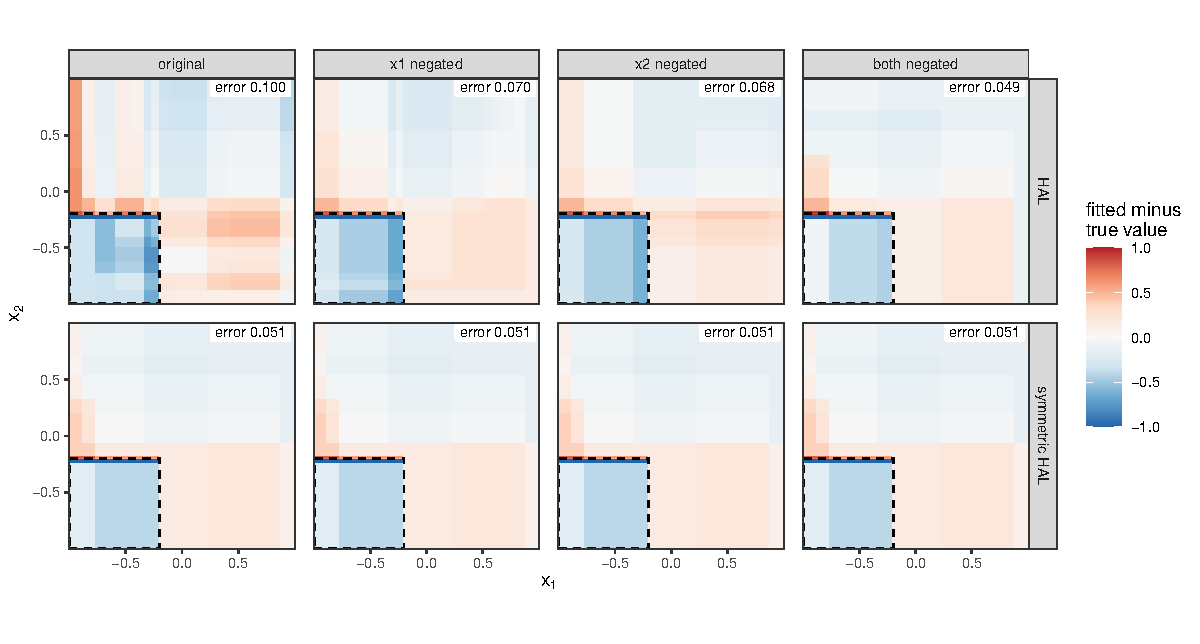
\includegraphics[width=\textwidth]{../figures/coding.pdf}
\caption{One data set ($n = 500$, true function $2$ on the dashed box, noise
SD $1.2$) fit under four sign codings of $(x_1, x_2)$, each drawn on the
original axes as fitted minus true value. Cross-validation folds are the
same in every fit. HAL's error halves as the coding turns the box toward its
anchor; symmetric HAL's fit is the same in every coding.}
\label{fig:coding}
\end{figure}

This paper makes the dependence exact and removes it.
\begin{enumerate}
\item \emph{The cost of orientation} (Section~\ref{sec:cost}). For a box
  with $m$ upper-sided, $k$ lower-sided and $t$ two-sided coordinates, the
  anchored penalty is $2^{t+k}$ (or $2^{t+k}-1$ for a lower orthant) times
  the box's height, while the smallest penalty available with both
  orientations is $2^t$ (Proposition~\ref{prop:box}). The lower bound comes
  from the Vitali variation and holds for any representation. Through a
  standard oracle inequality the same factor enters HAL's risk bound
  (Corollary~\ref{cor:orient}).
\item \emph{Coding invariance} (Section~\ref{sec:equiv}). Adding the
  reflected indicators $\one\{x_j \le u\}$ gives a dictionary that sign
  recoding maps onto itself. The resulting estimator, symmetric HAL, has
  identical fitted values when any covariate is negated
  (Proposition~\ref{prop:equiv}); HAL does not.
\item \emph{No loss in rate} (Section~\ref{sec:rates}). The symmetric
  variation class is a sum of $2^d$ reflected copies of the anchored class,
  so its metric entropy is within a constant of the anchored one. The
  constrained symmetric estimator inherits the $n^{-2/3}$ rate of
  \citet{fang2021} and is minimax rate optimal over its class
  (Proposition~\ref{prop:rate}).
\item \emph{Evidence} (Sections~\ref{sec:sims}--\ref{sec:semisynth}).
  Simulations across signal shapes and signal-to-noise ratios, with CART
  and random forests as references, measure the gap in risk rather than in
  bounds. Recoding the covariates of two prediction data sets and of
  LaLonde's benchmark measures it on real data, and a semi-synthetic
  version of the benchmark, with a known effect, measures bias, variance
  and coverage of the treatment-effect estimators.
\end{enumerate}

\paragraph{Related work.} That Hardy--Krause variation depends on an anchor
is known in quasi-Monte Carlo, where it is anchored at either corner
\citep{aistleitner2015}; \citet{fang2021} note the choice and fix the anchor
at $0$. Their near-parametric rate for HAL-type estimators is proved for
indicators of upper-right rectangles, the boxes that face the anchor. The
statistical consequences of the anchor for HAL, and an estimator free of it,
are to our knowledge new. Multivariate adaptive regression splines
\citep{friedman1991} use reflected pairs of hinge functions, $(x-t)_+$ and
$(t-x)_+$, for the same reason; symmetric HAL is the zero-order, convex
analogue. The lasso version of MARS \citep{ki2024} keeps only $(x-t)_+$,
noting that $(t-x)_+ = (x-t)_+ - x + t$ lies in its span; the span is the
same, but the penalty of a function is not, which is the subject of
Section~\ref{sec:cost}. First-order HAL, the \texttt{hal9001} default, likewise uses one-sided
hinges; we develop the theory for zero order and show in
Section~\ref{sec:real} that the default estimator is at least as sensitive
to the coding. The implementation in
\texttt{hal9001} \citep{hejazi2020} uses the anchored basis: we reproduce
its fits exactly. Regression trees \citep{breiman1984} have no such
dependence: a split at $c$ sends $x_j \ge c$ to one child and $x_j < c$ to
the other, so negating a covariate swaps the children and leaves the fit
unchanged. A tree is a greedy search over products of these two-sided
indicators \citep{friedman1991,klusowski2024}; symmetric HAL is the lasso
over the same set, of which HAL keeps one orientation.


\section{Setup}

Let $x \in \R^d$. For a \emph{section} $s \subseteq [d]$, a knot
$u \in \R^{s}$ and an \emph{orientation} $o \in \{+,-\}^{s}$, define the
feature
\[
  \phi_{s,u,o}(x) = \prod_{j \in s} h_{o_j}(x_j - u_j), \qquad
  h_+(t) = \one\{t \ge 0\}, \quad h_-(t) = \one\{t \le 0\}.
\]
The \emph{anchored dictionary} $\mathcal{A}$ contains the features with
$o \equiv +$; this is the zero-order basis of the Highly Adaptive Lasso
(HAL; \citealp{vanderlaan2017,benkeser2016}). The \emph{symmetric dictionary}
$\mathcal{S}$ contains all orientations. Both are restricted to
$1 \le |s| \le D$ and to knots on a grid $K = \prod_j K_j$.
Reflection $x_j \mapsto -x_j$ maps $\mathcal{S}$ onto itself (with
$K_j \mapsto -K_j$); it does not map $\mathcal{A}$ onto itself.

For a dictionary $\mathcal{D}$, the \emph{penalty} of a function $f$ is the
smallest $\ell_1$ norm over representations, with the constant unpenalized:
\[
  V_{\mathcal{D}}(f) = \inf\Big\{ \textstyle\sum_{\phi} |\beta_\phi| :
  f = \beta_0 + \sum_{\phi \in \mathcal{D}} \beta_\phi \phi \Big\},
\]
with $V_{\mathcal{D}}(f) = \infty$ if no representation exists. Since
$\mathcal{A} \subseteq \mathcal{S}$, $V_{\mathcal{S}} \le V_{\mathcal{A}}$.
For $\mathcal{A}$ the representation is unique (the anchored features with
distinct $(s,u)$ are linearly independent together with the constant), so
$V_{\mathcal{A}}(f)$ is the $\ell_1$ norm of the coefficients; on
$[0,1]^d$ with knots everywhere it is the sectional (Hardy--Krause)
variation anchored at the lower corner \citep{vanderlaan2017}.

Given data $(x_i, y_i)_{i=1}^n$ and a finite dictionary with design
$X \in \R^{n \times p}$, the lasso estimator is
\begin{equation}\label{eq:lasso}
  (\hat\beta_0, \hat\beta) \in \argmin_{\beta_0,\beta}
  \tfrac{1}{2n}\|y - \beta_0\one - X\beta\|_2^2 + \lambda \|\beta\|_1 .
\end{equation}
HAL is \eqref{eq:lasso} on $\mathcal{A}$; \emph{symmetric HAL} is
\eqref{eq:lasso} on $\mathcal{S}$.

\section{What a box costs}\label{sec:cost}

A box $B = \prod_{j \in s} I_j$ in section $s$ has, in each coordinate,
an interval $I_j$ that is \emph{upper} ($[a_j,\infty)$), \emph{lower}
($(-\infty,b_j]$) or \emph{two-sided} ($[a_j,b_j]$). Let $m,k,t$ count
the upper, lower and two-sided coordinates, $m+k+t=|s|$, with $|s| \le D$.
Take the domain to be a finite grid $G = \prod_j G_j$, such as a lattice
design or the observed values, with a knot at every grid point, so that
$\one\{x_j > b\} = h_+(x_j - b^+)$ where $b^+$ is the next point of $G_j$
above $b$; finite endpoints lie in $G$.

\begin{proposition}[Penalty of a box]\label{prop:box}
For $f = c\,\one_B$ with $c \neq 0$,
\[
  V_{\mathcal{S}}(f) = |c|\, 2^{t}, \qquad
  V_{\mathcal{A}}(f) = |c| \big(2^{t+k} - \one\{m = t = 0\}\big).
\]
In particular, for an orthant ($t = 0$) $V_{\mathcal{S}}(f) = |c|$ for
every orientation, while $V_{\mathcal{A}}(f)$ ranges from $|c|$ (upper
orthant) to $|c|(2^{|s|}-1)$ (lower orthant).
\end{proposition}

\begin{proof}
\emph{Anchored value.} Write $\one\{x_j \le b\} = 1 - h_+(x_j - b')$ where
$b' = b^+$ is the next grid point above $b$, and
$\one\{a \le x_j \le b\} = h_+(x_j - a) - h_+(x_j - b')$. Expanding the
product over $j \in s$ gives one term per choice of a summand from each
factor: one choice for upper coordinates and two for lower and two-sided
coordinates, so $2^{t+k}$ terms, each $\pm c$ times a distinct anchored
feature or, exactly when every factor contributes its constant $1$, the
constant. The constant is available only if $m = t = 0$. By uniqueness of
the anchored representation, $V_{\mathcal{A}}(f)$ is the sum of
$|{\pm c}|$ over the non-constant terms.

\emph{Symmetric upper bound.} Use the oriented indicator directly for each
one-sided coordinate and $h_+(x_j - a_j) - h_+(x_j - b_j')$ for each
two-sided one: $2^t$ features with coefficients $\pm c$.

\emph{Lower bound.} Fix the coordinates outside $s$ at values inside $B$'s
projection. On the resulting $|s|$-dimensional slice consider the grid
generated by the finite endpoints of $B$ and points just outside them, and
the Vitali variation (sum over grid cells of the absolute $|s|$-th mixed
difference). For $f = c\,\one_B$ it equals $|c|$ times the number of
finite corners of $B$ in $s$, which is $2^t$. Every feature
$\phi_{s',u,o}$ restricted to the slice either does not depend on some
coordinate in $s$ (if $s \not\subseteq s'$), so all its mixed differences
vanish, or is $0/1$ times a product of $|s|$ monotone one-jump indicators,
whose Vitali variation is at most $1$. The Vitali variation is a seminorm
that vanishes on constants, so for any representation
$2^t |c| \le \sum_\phi |\beta_\phi|$. This proves
$V_{\mathcal{S}}(f) \ge 2^t |c|$ and, as $V_{\mathcal{A}} \ge V_{\mathcal{S}}$,
the anchored lower bound in the case $k = 0$; for $k>0$ the anchored value
was already exact.
\end{proof}

\begin{theorem}[Slow-rate oracle inequality]\label{thm:oracle}
Let $y_i = f^*(x_i) + \varepsilon_i$ with fixed design and independent
mean-zero $\sigma$-sub-Gaussian $\varepsilon_i$. Let $X$ be any design with
$\|X_{\cdot j}\|_2^2 / n \le 1$, let $P = I - \one\one^\top/n$ and
$\|g\|_{n,c}^2 = \|Pg\|_2^2/n$. If
$\lambda \ge 2 \|(PX)^\top \varepsilon\|_\infty / n$, then any solution of
\eqref{eq:lasso} satisfies, for every $\beta$,
\[
  \|\hat f - f^*\|_{n,c}^2 \le \|f_\beta - f^*\|_{n,c}^2 + 3\lambda\|\beta\|_1 .
\]
The condition on $\lambda$ holds with probability at least $1-\delta$ for
$\lambda = 2\sigma\sqrt{2\log(2p/\delta)/n}$.
\end{theorem}

\begin{proof}
Profiling out $\beta_0$ turns \eqref{eq:lasso} into the lasso on $(Py, PX)$.
Comparing the objective at $\hat\beta$ and at $\beta$ and substituting
$Py = Pf^* + P\varepsilon$,
\[
  \tfrac{1}{2n}\|P(f^* - X\hat\beta)\|^2 \le
  \tfrac{1}{2n}\|P(f^* - X\beta)\|^2
  + \tfrac{1}{n}\varepsilon^\top PX(\hat\beta - \beta)
  + \lambda\|\beta\|_1 - \lambda\|\hat\beta\|_1 .
\]
The middle term is at most
$\tfrac{\lambda}{2}(\|\hat\beta\|_1 + \|\beta\|_1)$ by H\"older's inequality
and the condition on $\lambda$. Rearranging and multiplying by $2$ gives the
claim. For the probability, $(PX_{\cdot j})^\top\varepsilon / n$ is
sub-Gaussian with variance proxy $\sigma^2 \|PX_{\cdot j}\|^2/n^2 \le
\sigma^2/n$; a union bound over $p$ columns finishes.
\end{proof}

Indicator columns satisfy the normalization. With $D$ the maximal degree and
$q$ knots per coordinate, $p_{\mathcal{A}} = \sum_{r \le D}\binom{d}{r}q^r$
and $p_{\mathcal{S}} \le 2^D p_{\mathcal{A}}$, so the two choices of
$\lambda$ differ by at most a factor
$\sqrt{1 + D\log 2 / \log(2p_{\mathcal{A}}/\delta)}$.

\begin{corollary}[Misoriented boxes]\label{cor:orient}
If $f^* = c\,\one_B$ for an orthant $B$ with $k$ lower coordinates
($t=0$, $m \ge 1$), the bound of Theorem~\ref{thm:oracle} is
$3\lambda_{\mathcal{A}} 2^k |c|$ for HAL and $3\lambda_{\mathcal{S}} |c|$ for
symmetric HAL. For the lower orthant ($m=0$) the HAL bound is
$3\lambda_{\mathcal{A}}(2^{|s|}-1)|c|$.
\end{corollary}

\begin{remark}
These are upper bounds; the corollary does not show that HAL's risk is
larger. The simulations in Section~\ref{sec:sims} test whether the gap
appears in risk.
\end{remark}

\section{Coding invariance}\label{sec:equiv}

Whether a covariate is recorded as $x_j$ or $-x_j$ (age or years to
retirement, a dose or its distance from a maximum) is usually arbitrary.
Let $R_j$ negate coordinate $j$. Call a knot rule \emph{reflection
equivariant} if the knots computed from $R_j$-reflected data are the
negated knots; sample quantiles at a set of probability levels closed under
$p \mapsto 1-p$ qualify (for the type-7 quantile,
$Q_{-x}(p) = -Q_x(1-p)$). Call a column filter reflection equivariant if
it keeps a column exactly when it keeps its reflection; filters that act on
the share of ones and on duplicate columns qualify, provided a column and
its complement are treated alike.

\begin{proposition}[Reflection equivariance]\label{prop:equiv}
Let the knot rule and the column filter be reflection equivariant. Then the
symmetric dictionary built from reflected data
$\{(R_j x_i, y_i)\}$ spans, together with the constant, the reflections
$\{\phi \circ R_j\}$ of the dictionary built from $\{(x_i, y_i)\}$, with
the same penalty: $V_{\mathcal{S}}^{R_j\text{-data}}(f \circ R_j) =
V_{\mathcal{S}}(f)$. Consequently the fitted values of symmetric HAL at any
fixed $\lambda$ are identical on the two data sets, and when the lasso
solution is unique the fitted functions satisfy
$\hat f^{R_j} = \hat f \circ R_j$. The anchored dictionary has neither
property.
\end{proposition}

\begin{proof}
For a feature with $j \in s$,
$\phi_{s,u,o}(R_j x) = \phi_{s,u',o'}(x)$ with $u'_j = -u_j$,
$o'_j = -o_j$ and the other entries unchanged, because
$h_{o_j}(-x_j - u_j) = h_{-o_j}(x_j + u_j)$. So $\phi \mapsto \phi \circ R_j$
is a bijection between the dictionary features at knots $K$ and at knots
$R_j K$ with orientations flipped in coordinate $j$; the symmetric
dictionary contains both orientations, so it is mapped onto itself. This
includes main effects: storing only $h_+$ main effects and relying on
$h_-(x_j - u) = 1 - h_+(x_j - u^+)$ requires the next data value $u^+$
above $u$ to be a knot, which fails when knots fall on tied data values,
so the symmetric dictionary keeps both orientations of each main effect.
Duplicate columns, and pairs of columns that sum to the constant, add no
cheaper representations: $\beta_1\phi + \beta_2(1-\phi) = \beta_2 +
(\beta_1 - \beta_2)\phi$ and $|\beta_1| + |\beta_2| \ge |\beta_1 - \beta_2|$,
with the constant unpenalized. The equivariant knot rule and filter make the
two retained column sets correspond under this bijection. The lasso
objective depends on the design only through the column set (up to order)
and the span of the unpenalized constant, so the two problems are the same
problem after relabelling columns; lasso fitted values are unique
\citep{tibshirani2013}, which gives the first consequence, and with a
unique solution the coefficients correspond, which gives the second. For
the anchored dictionary, $\one\{x_j \ge u\}\one\{x_l \ge v\}$ becomes a
lower-orthant feature in coordinate $j$ after reflection, which the
anchored dictionary represents only with three features
(Proposition~\ref{prop:box}), so the penalties differ.
\end{proof}

The numeric check in the repository fits both estimators at a fixed
$\lambda$ to data and to data with one coordinate negated: the symmetric
fits agree to solver tolerance ($4 \times 10^{-7}$), while the anchored fits
differ by up to $0.2$ on an outcome whose signal has range $1.5$.

\section{Rates}\label{sec:rates}

\citet{fang2021} study the constrained estimator
$\hat f_{\mathcal{A},V} \in \argmin\{\sum_i (y_i - f(x_i))^2 :
V_{\mathcal{A}}(f) \le V\}$ on the lattice design
$\{(i_1/n_1, \ldots, i_d/n_d)\}$ with knots at all lattice points and
$D = d$, and prove (their Theorem 4.5) that if $V \ge V_{\mathcal{A}}(f^*)$,
\begin{equation}\label{eq:fgs}
  \tfrac{1}{n}\mathbb{E}\textstyle\sum_i (\hat f(x_i) - f^*(x_i))^2
  \le C_d \Big(\frac{\sigma^2 V}{n}\Big)^{2/3}
  \Big(\log\big(2 + \tfrac{V\sqrt{n}}{\sigma}\big)\Big)^{\frac{2d-1}{3}}
  + C_d \frac{\sigma^2}{n},
\end{equation}
with a matching minimax lower bound up to logarithmic factors over
$\{V_{\mathcal{A}} \le V\}$ (their Theorem 4.6; theorem and lemma numbers refer to the arXiv version,
1903.01395v3). Define
$\hat f_{\mathcal{S},V}$ in the same way with $V_{\mathcal{S}}$.

\begin{proposition}[Symmetric rate]\label{prop:rate}
If $V \ge V_{\mathcal{S}}(f^*)$, $\hat f_{\mathcal{S},V}$ satisfies
\eqref{eq:fgs} with $C_d$ replaced by a constant $C'_d$ depending only on
$d$. Since $\{V_{\mathcal{A}} \le V\} \subseteq \{V_{\mathcal{S}} \le V\}$,
the minimax lower bound of \citet{fang2021} applies to the symmetric class,
so $\hat f_{\mathcal{S},V}$ is minimax rate optimal over it up to
logarithmic factors.
\end{proposition}

\begin{proof}
The proof of \citet[Section~8.4]{fang2021} uses two facts about the
constraint set $C(V) = \{(f(x_1), \ldots, f(x_n)) : V_{\mathcal{A}}(f) \le V\}$:
it is closed and convex, and its intersection with a Euclidean ball,
$C(V, t) = C(V) \cap B_2(0, t)$, has covering numbers bounded as in their
Lemma 8.6,
\[
  \log N(\epsilon, C(V, t)) \le C_d \Big(\big(\tfrac{V\sqrt{n}}{\epsilon}
  \big)^{1/2} + 1\Big)\Big(\log\big(\tfrac{2V\sqrt{n}}{\epsilon} + 1\big)
  \Big)^{d - \frac12} + \log\Big(2 + 2\,\tfrac{t + V\sqrt{n}}{\epsilon}\Big).
\]
The rest of their argument depends on $C(V)$ only through this bound. The
symmetric set $C_{\mathcal{S}}(V)$ is closed and convex (an $\ell_1$ ball
image plus the constant direction). For an orientation pattern
$r \in \{+,-\}^d$, the features with orientation $r$ on their section
are, on the lattice, the anchored features composed with the reflection
that reverses the lattice index in the coordinates where $r_j = -$, after
the knot relabelling of Proposition~\ref{prop:equiv}; that reflection is a
permutation $P_r$ of the $n$ coordinates. Group the terms of any
representation by orientation pattern and give the whole constant to
$r = (+,\ldots,+)$. Then every $\theta \in C_{\mathcal{S}}(V) \cap B_2(0,t)$
is $\sum_r P_r \theta_r$ with $\theta_r \in C(V)$; for
$r \neq (+,\ldots,+)$, $\theta_r$ has no constant term, so
$\|\theta_r\|_\infty \le V$ and $\|\theta_r\|_2 \le V\sqrt{n}$, and hence
the constant-carrying component has $\|\theta_{+}\|_2 \le
t + 2^d V\sqrt{n}$. Permutations preserve Euclidean covering numbers, and
an $\epsilon 2^{-d}$-cover of each of the $2^d$ pieces gives an
$\epsilon$-cover of the sum, so
\[
  \log N(\epsilon, C_{\mathcal{S}}(V, t)) \le 2^d
  \log N\big(\epsilon 2^{-d}, C(V, t + 2^d V\sqrt{n})\big).
\]
Substituting Lemma 8.6 changes only constants and the argument of the
last logarithm, which enters the final bound only through a term of order
$t\sqrt{\log(4 + c_d V\sqrt n / t)}$, as in their proof. Following their
argument with this bound gives \eqref{eq:fgs} with a new constant.
\end{proof}

Combining Propositions~\ref{prop:box} and~\ref{prop:rate}: for a lower
orthant box in a $|s|$-dimensional section, the oracle-tuned anchored
bound is $(2^{|s|}-1)^{2/3}$ times the symmetric bound in its leading term,
$2.08$ for $|s| = 2$, and $2^{2k/3}$ times for an orthant with $k < |s|$
lower coordinates, $1.59$ for $k = 1$. As with Corollary~\ref{cor:orient}
these compare upper bounds. \citet{fang2021} also prove a near-parametric
rate for the anchored estimator on indicators of upper-right rectangles
(their Theorems 4.7 and 6.1). We do not prove the reflected statement for
$\hat f_{\mathcal{S},V}$, whose tangent cones differ.

\section{Computation}\label{sec:comp}

The symmetric dictionary has $2^{|s|}$ times as many features as the
anchored one in each section $s$; for main effects the extra orientation
matters only when knots fall on tied data values, but it is needed there
for exact equivariance. With the screening HAL already applies (drop indicators that
are nonzero for fewer than $\sqrt{n}$ observations), at $n = 500$, $d = 10$,
nine knots per coordinate and $D = 2$, the anchored dictionary has $3{,}389$
columns and the symmetric one $13{,}368$. The estimator is an ordinary lasso
on that design; we use \texttt{glmnet} with cross-validated $\lambda$ and no
standardization, so the coefficient $\ell_1$ norm is the penalty of
Section~\ref{sec:cost}. No new software is needed: \texttt{hal9001}
accepts a user-supplied basis, and on the design $(x, -x)$ its indicator
$\one\{-x_j \ge -u\}$ is $h_-(x_j - u)$, so passing it the symmetric basis
with each lower-sided coordinate moved to the negated copy fits symmetric
HAL with all of its families and tuning options. The accompanying code does
this and checks that the fitted values match the direct lasso.

\section{Simulations}\label{sec:sims}

\paragraph{Design.} Covariates are $d = 10$ independent uniforms on
$[-1,1]$, $n = 500$, and Gaussian noise is set to signal-to-noise ratios
(signal variance over noise variance) from $0.05$ to $4$, with 50
replicates per cell. The regression functions are a $2$-D box of height $2$
in each orientation (upper, mixed and lower orthant, and interior), a sum of
eight boxes in random orthant orientations, a depth-two tree, an additive
step function whose three steps all switch on as their covariate increases,
XOR, and Friedman's smooth function. Methods: HAL, symmetric HAL, both also
with a relaxed refit, and, as references, CART pruned by cross-validation and
a random forest. Both dictionaries use nine sample-quantile knots per
coordinate, degree $D = 2$ and the same screening; $\lambda$ is chosen by
10-fold cross-validation. Risk is measured on 2{,}000 fixed test points and
reported relative to the risk of the constant predictor; comparisons between
methods are paired within replicate.

\paragraph{Predictions stated before the runs.} (i) Symmetric HAL and HAL tie
on the upper-orthant and interior boxes, where Proposition~\ref{prop:box}
gives equal penalties. (ii) Symmetric HAL wins on the mixed and lower boxes,
by more on the lower box. (iii) Symmetric HAL does equally well on a box and
on its reflection (Proposition~\ref{prop:equiv}).

\paragraph{Results.} Table~\ref{tab:tier1_ratio} gives the median risk ratio
of symmetric HAL to HAL and Figure~\ref{fig:orientation} every replicate.
Prediction (ii) holds: on the lower box symmetric HAL's risk is $0.44$ times
HAL's at signal-to-noise $0.25$, and on the mixed box $0.59$ times, and it is
lower in every replicate at signal-to-noise $0.25$ to $4$. The gap is largest
at moderate noise and narrows at both ends, where either both fits are close
to the constant or both have enough data to pay for the extra terms.

Prediction (i) fails. On the upper box HAL is better at every
signal-to-noise ratio, by $3$ to $18\%$ in median risk; on the interior box
symmetric HAL is better at low signal-to-noise and $18$ to $20\%$ worse at
high. Both boxes cost the same in the two dictionaries, so the difference is
the price of a dictionary four times larger in the interactions, which
Theorem~\ref{thm:oracle} sees only through a logarithmic factor. The relaxed
refit, which removes the lasso's shrinkage from the selected terms, removes
most of this price: the relaxed fits tie on the upper box from
signal-to-noise $0.5$ upward (ratio $1.00$). The additive truth behaves like
the upper box, as its steps all face HAL's anchor, with symmetric HAL up to
$15\%$ worse. Where no orientation is privileged, symmetric HAL is better:
on the eight randomly oriented boxes its risk is $0.64$ times HAL's at high
signal-to-noise, on the tree $0.73$ to $0.97$ times, on XOR $0.61$ to $0.95$
times, and on Friedman's smooth function within $7\%$ either way.

Prediction (iii) holds for each data set but cannot be read off the risk
distributions. Fitting the upper box and its exact mirror image (data and test
points reflected) gives the same risk up to solver tolerance (three
replicates at signal-to-noise $2$: $0.0912$ and $0.0912$, $0.1669$ and
$0.1671$, $0.1354$ and $0.1354$), as Proposition~\ref{prop:equiv}
requires. The lower-box risks in the grid are higher than the upper-box ones
at high signal-to-noise because the same test points are used for both and
they are not mirror symmetric: at high signal-to-noise the error sits in thin
bands along the box edges, which contain few test points.

The references behave as expected from their structure
(Appendix Figure~\ref{fig:all_methods}). CART, which needs
only two splits for a box, has lower risk than relaxed symmetric HAL on the
single boxes and the tree at most signal-to-noise ratios; on the eight boxes,
XOR and Friedman's function it is worse, by up to a factor of $6$ at high
signal-to-noise. Symmetric HAL
took a median of $8$ seconds per fit, HAL $4$.

\begin{table}[!h]
\centering
\caption{\label{tab:tier1_ratio}Risk of symmetric HAL relative to HAL, by true function (rows) and signal-to-noise ratio (columns): the median over 50 replicates of the within-replicate ratio. Below 1, symmetric HAL is better.}
\centering
\begin{tabular}[t]{lrrrrrrr}
\toprule
\multicolumn{1}{c}{ } & \multicolumn{7}{c}{signal-to-noise ratio} \\
\cmidrule(l{3pt}r{3pt}){2-8}
true function & 0.05 & 0.1 & 0.25 & 0.5 & 1 & 2 & 4\\
\midrule
tree & 0.97 & 0.91 & 0.81 & 0.80 & 0.75 & 0.73 & 0.76\\
additive steps & 0.89 & 0.93 & 0.97 & 1.02 & 1.08 & 1.15 & 1.15\\
XOR & 0.95 & 0.71 & 0.61 & 0.63 & 0.69 & 0.77 & 0.83\\
upper box & 1.09 & 1.18 & 1.16 & 1.10 & 1.06 & 1.05 & 1.03\\
mixed box & 0.92 & 0.71 & 0.59 & 0.62 & 0.66 & 0.78 & 0.82\\
lower box & 0.97 & 0.68 & 0.44 & 0.45 & 0.55 & 0.65 & 0.74\\
interior box & 0.99 & 0.89 & 0.87 & 0.88 & 1.03 & 1.20 & 1.18\\
eight boxes & 1.00 & 0.98 & 0.95 & 0.85 & 0.76 & 0.65 & 0.64\\
Friedman & 1.01 & 1.03 & 0.96 & 0.93 & 0.93 & 0.93 & 0.97\\
\bottomrule
\end{tabular}
\end{table}


\begin{figure}[!h]
\centering
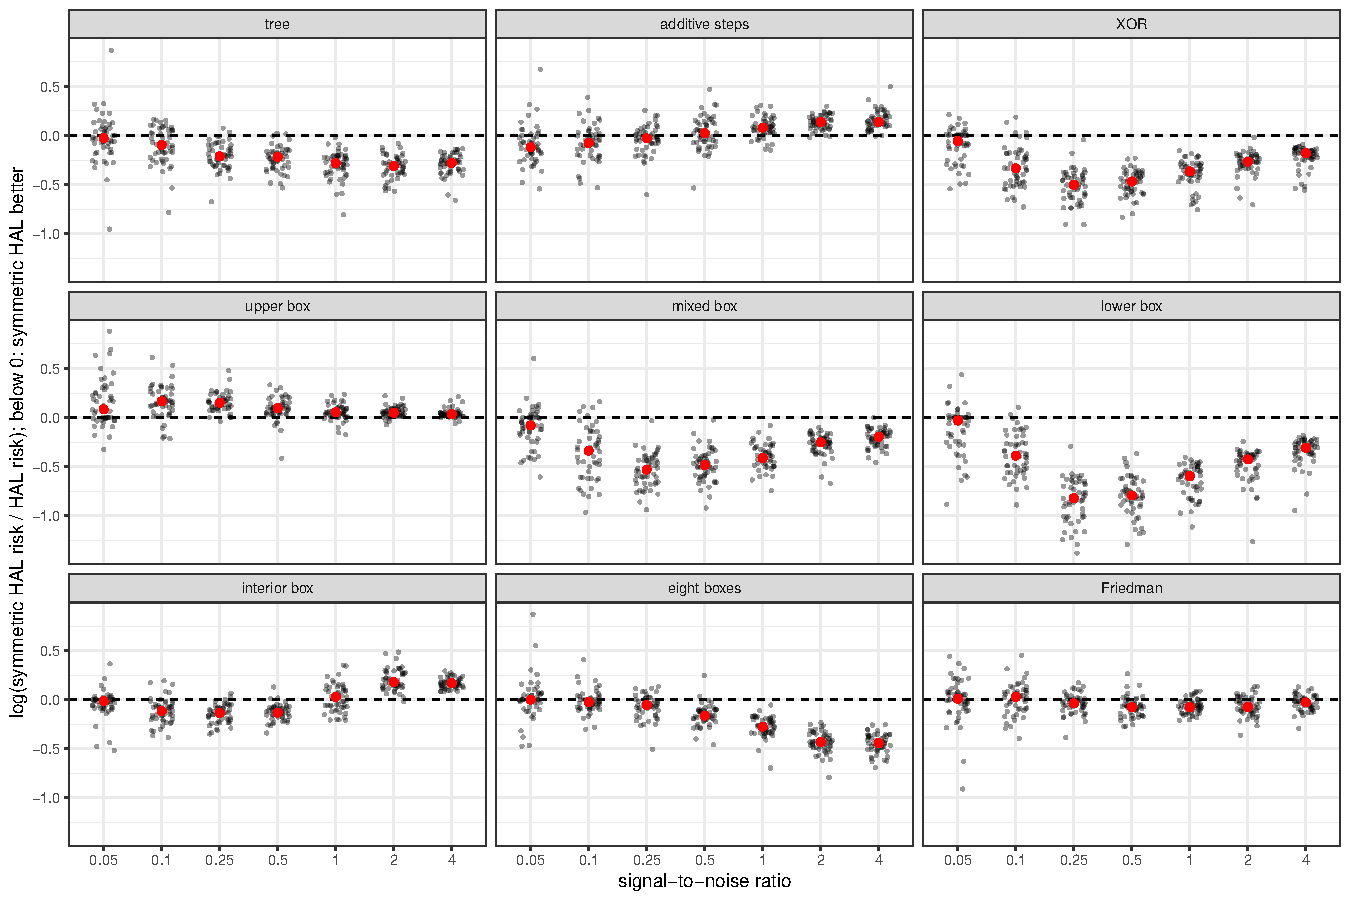
\includegraphics[width=\textwidth]{../figures/tier1_p1_orientation.pdf}
\caption{Log risk ratio of symmetric HAL to HAL in each of 50 replicates
(points) and its median (red), by true function and signal-to-noise ratio.
Below zero, symmetric HAL is better.}
\label{fig:orientation}
\end{figure}

\section{Recoding real covariates}\label{sec:real}

The propositions say the coding matters for HAL; this section measures how
much on real data. For each data set we take the original coding and 20
random recodings, each negating every covariate independently with
probability $1/2$, and refit HAL and symmetric HAL with everything else
held fixed: the same knot rule, the same cross-validation folds, and the
same test split. A negated covariate carries exactly the information the
original did, so any change in the output is due to the coding alone. We
use a tight solver tolerance (\texttt{glmnet} threshold $10^{-12}$); at the
default tolerance, near-ties in the cross-validation curve let equivalent
codings select different $\lambda$, which is a solver artefact rather than a
property of the estimator.

\paragraph{Prediction.} Boston housing (13 covariates, median home value)
and Los Angeles ozone (9 covariates, daily maximum ozone) are split once
into 70\% training and 30\% test rows. Table~\ref{tab:recode_predictions}
reports, for each test point, the spread of its prediction across the 21
codings. Under HAL a typical test prediction moves by $0.11$ outcome
standard deviations across codings, and some move by more than one
standard deviation. Test error ranges from $2.59$ to $3.26$ on Boston and
from $4.82$ to $5.59$ on ozone, depending only on which way the covariates
point. Symmetric HAL's predictions agree across codings to within
$0.003$ standard deviations, the residual being solver tolerance. Its test
error sits near the median of HAL's: the coding-free estimator is not more
accurate than a typical coding, and the best coding of HAL is better on
Boston. That coding cannot be picked without the test set, and no analyst
would think to search for it.

\begin{table}[!h]
\centering
\caption{\label{tab:recode_predictions}Predictions across random sign codings of the covariates, on a fixed test set of 30 percent of the rows. Mean SD and max range are per test point, in units of the outcome's standard deviation.}
\centering
\begin{tabular}[t]{llrrrrrr}
\toprule
Data & Method & Codings & Mean SD & Max range & RMSE min & RMSE median & RMSE max\\
\midrule
Boston & HAL, zero order & 21 & 0.115 & 1.298 & 2.585 & 2.888 & 3.258\\
Boston & symmetric HAL & 21 & 0.000 & 0.000 & 2.973 & 2.973 & 2.973\\
Ozone & HAL, zero order & 21 & 0.108 & 1.082 & 4.820 & 5.171 & 5.589\\
Ozone & symmetric HAL & 21 & 0.000 & 0.003 & 5.123 & 5.123 & 5.123\\
\bottomrule
\end{tabular}
\end{table}


\paragraph{A treatment effect.} The case that motivates the paper is HAL
as a nuisance estimator, and the classic test of a nuisance estimator is
\citet{lalonde1986}'s: estimate the effect of a job-training program from
observational data and compare the answer with the program's own randomized
experiment. We use the \citet{dehejia1999} sample of the National Supported
Work (NSW) program: 185 trainees, whose experimental control group of 260
gives an effect on 1978 earnings of \$1{,}794 (standard error \$671), and
2{,}490 non-experimental comparison individuals from the Panel Study of
Income Dynamics (PSID-1). The covariates are age, education, two race
indicators, marital status, no high-school degree, and 1974 and 1975
earnings. The target is the average effect on the treated, estimated by the
cross-fitted augmented inverse-probability-weighted estimator
\citep{chernozhukov2018} over five folds: the outcome regression is fit on
the comparison group, the propensity score on everyone, the latter capped at
$0.99$, and each nuisance function is tuned by cross-validation on folds that
are fixed across codings.

We fit the nuisance functions four ways. Most applied work runs
\texttt{hal9001} with its defaults, which are first-order HAL: one-sided
hinges $(x_j - u)_+$ and their products up to degree three, with 50, 25 and
12 knots per coordinate for degrees one to three. The symmetric first-order
fit adds the reflected hinges $(u - x_j)_+$ through the route of
Section~\ref{sec:comp}, with knots placed at quantiles that are symmetric
under negation (\texttt{hal9001} places its knots at quantiles of the
lower $98\%$ of each covariate, which a recoding moves). The zero-order fits
are those of Section~\ref{sec:sims}.

Table~\ref{tab:lalonde_att} and Figure~\ref{fig:lalonde_att} give the 19
distinct codings (two of the 20 random sign patterns repeated). With the
default fits the estimate runs from $-\$16{,}526$ to \$1{,}849, a range of
$18$ standard errors; leaving out the most extreme coding it still runs from
$-\$5{,}240$ to \$1{,}849, and it is negative in 9 of the 19 codings. The
coding moves the propensity fit as well as the outcome fit: in three
codings, including the original one, some comparison individual reaches the
$0.99$ cap, and the standard error triples. Zero-order HAL is less
sensitive, from \$451 to \$3{,}551 (2.6 standard errors). Both symmetric
estimators are flat: \$1{,}852 to \$1{,}903 with first-order fits, and
\$2{,}800 in every coding with zero-order fits. The symmetric first-order basis is the same set of columns in every
coding (we check this on these data), so by the argument of
Proposition~\ref{prop:equiv}
the exact fit is too, and the remaining spread, $0.05$ standard errors, is
the solver's convergence tolerance; we keep \texttt{glmnet}'s default tolerance for these fits
because a tighter one stops the cross-validation path early.

This is evidence about coding, not about which estimator is right. The
symmetric first-order estimate is \$79 from the experimental benchmark and
the zero-order one \$1{,}006 from it, but the benchmark's own standard
error is \$671, and agreement with one experiment is weak evidence of
accuracy: these data are notorious for estimates that change with the
specification \citep{smith2005}. Removing the dependence on coding fixes
one of the specification choices; it does not make the remaining ones
right. Section~\ref{sec:semisynth} measures bias and variance where the
truth is known.

\begin{table}[!h]
\centering
\caption{\label{tab:lalonde_att}Cross-fitted AIPW estimates of the effect of NSW training on 1978 earnings of the treated (dollars), from the 185 trainees and the PSID-1 comparison group, across random sign codings of the eight covariates. Range / SE is the range divided by the median standard error; median distance is from the experimental estimate, 1,794 (SE 671).}
\centering
\resizebox{\ifdim\width>\linewidth\linewidth\else\width\fi}{!}{
\begin{tabular}[t]{lrrrrrrr}
\toprule
Nuisance fits & Codings & Min & Median & Max & Range / SE & Median SE & Median distance\\
\midrule
HAL, hal9001 defaults & 19 & -16,526 & 954 & 1,849 & 17.80 & 1,032 & 840\\
symmetric HAL, first order & 19 & 1,852 & 1,873 & 1,903 & 0.05 & 1,122 & 79\\
HAL, zero order & 19 & 451 & 2,251 & 3,551 & 2.60 & 1,194 & 934\\
symmetric HAL, zero order & 19 & 2,782 & 2,800 & 2,800 & 0.01 & 1,256 & 1,006\\
\bottomrule
\end{tabular}}
\end{table}


\begin{figure}[!h]
\centering
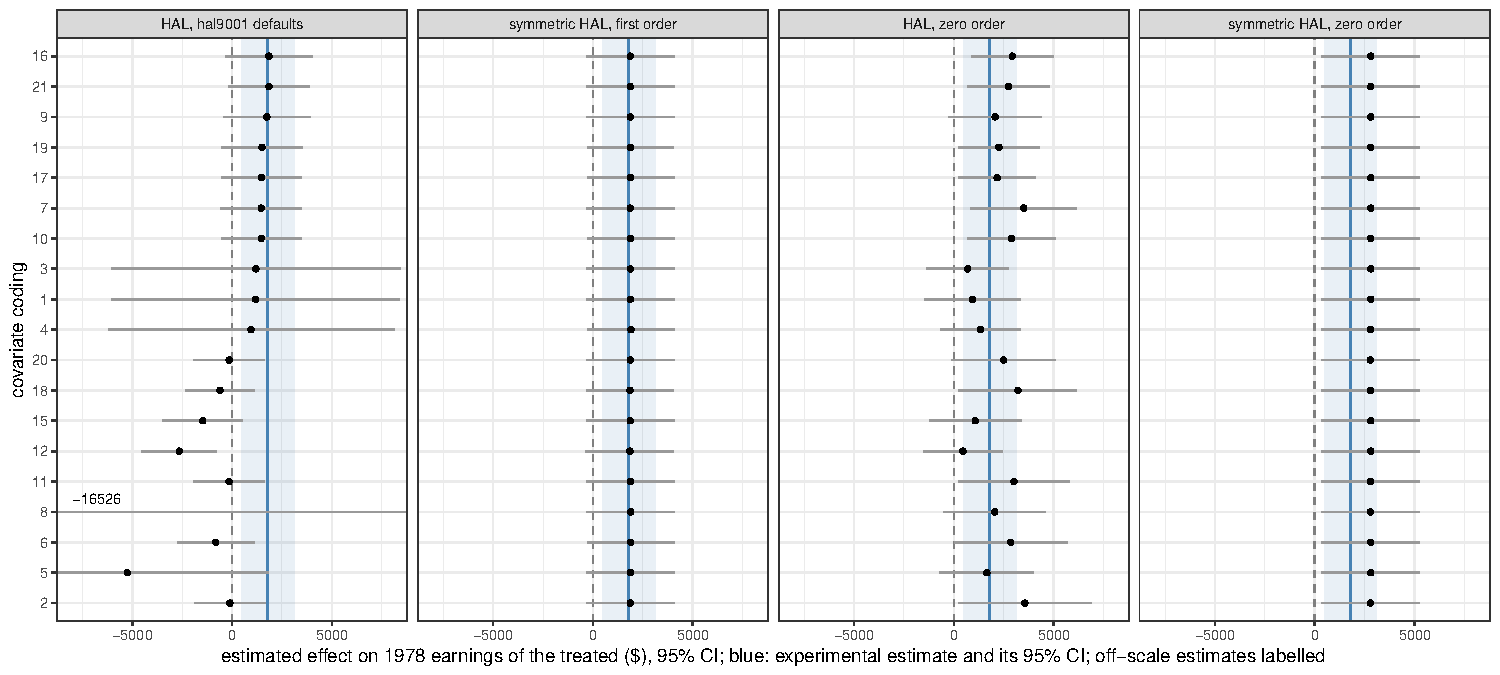
\includegraphics[width=\textwidth]{../figures/lalonde_att.pdf}
\caption{Estimates of the effect of NSW training on 1978 earnings of the
trainees, from the trainees and the PSID-1 comparison group, with 95\%
intervals, under the original coding (1) and 18 further distinct sign
codings of the covariates. Blue: the experimental estimate and its 95\%
interval. Codings are sorted by the default \texttt{hal9001} estimate; one
estimate lies off the scale and is labelled.}
\label{fig:lalonde_att}
\end{figure}

\section{Bias and variance with a known effect}\label{sec:semisynth}

LaLonde's comparison has one experiment to check against. To measure bias,
variance and coverage we keep the LaLonde covariates and replace the
treatment and the outcome with draws from known functions fitted to the
same data. Each replicate resamples the 2{,}675 trainees and comparison
individuals with replacement, draws treatment from the \citet{dehejia1999}
propensity logit (age and its square, education, the race, marital and
degree indicators, both earnings, and indicators of zero earnings in each
year), capped at $0.95$, and draws 1978 earnings as a fitted function of
the covariates for the comparison group (natural splines in age and both
earnings, the indicators, and the zero-earnings steps; $R^2 = 0.57$), plus
\$1{,}800 for the treated, plus Gaussian noise with the residual standard
deviation, \$10{,}190. About 180 individuals per replicate are treated, as
in the data, and the raw difference in mean earnings is around
$-\$14{,}000$, so the confounding is as severe as in the original. The
effect on the treated is \$1{,}800 by construction, and since the effect is
constant and the noise homoskedastic, the efficiency bound for the
estimator's standard deviation is
$\sigma \{E[g/(1-g)]\}^{1/2} / (p \sqrt{n})$, where $g$ is the propensity
score and $p$ the share treated, about \$2{,}300.

Each replicate is estimated twice, under the original coding and with the
four continuous covariates (age, education and both earnings) negated, with
the estimator and folds of Section~\ref{sec:real} and nuisance fits from
default \texttt{hal9001} and from symmetric first-order HAL. The two
codings carry the same information, so an estimator's answer should not
depend on which one it is given; across replicates we also get each
estimator's bias, its standard deviation against the bound, and the
coverage of its 95\% interval.

Table~\ref{tab:semisynth} and Figure~\ref{fig:semisynth} give 66
replicates. With the default fits the coding decides whether the estimator
works. Under the original coding it is biased by $-\$2{,}058$ (Monte Carlo
standard error about \$150), and its 95\% interval covers the truth in
$36\%$ of replicates. Its standard deviation, \$1{,}207, is half the
efficiency bound, below what any regular estimator can attain
asymptotically: the estimate is precise about the wrong number, and its standard error, which matches that
spread, cannot reveal the bias. Negating the four continuous covariates
removes the bias ($\$97$) and restores coverage ($94\%$) but makes the
estimator $1.3$ times as variable as the bound. Within a replicate the
estimate moves by a median of \$2{,}014 between the two codings, more than
the effect itself. With symmetric first-order fits the bias is
$-\$17$ and $-\$19$ in the two codings (Monte Carlo standard error about
\$270), the standard deviation is $0.95$ times the bound, coverage is
$97\%$, and the median move between codings is \$11. A standard deviation
at or slightly below the bound is within Monte Carlo error of it (the ratio
is estimated to about $\pm 9\%$); the cap on the estimated propensity score
can also trim variance at the cost of a little bias.

\begin{table}[!h]
\centering
\caption{\label{tab:semisynth}Semi-synthetic LaLonde: estimates of an effect on the treated of 1,800 dollars. SD / bound divides the standard deviation across replicates by the efficiency bound; coverage is that of the nominal 95 percent interval; median move is the median absolute change in the estimate between the two codings of the same replicate.}
\centering
\resizebox{\ifdim\width>\linewidth\linewidth\else\width\fi}{!}{
\begin{tabular}[t]{llrrrrrrrr}
\toprule
Nuisance fits & Coding & Reps & Bias & SD & RMSE & SD / bound & Mean SE & Coverage & Median move\\
\midrule
HAL, hal9001 defaults & original & 66 & -2,058 & 1,207 & 2,381 & 0.53 & 1,029 & 0.36 & 2,014\\
HAL, hal9001 defaults & continuous covariates negated & 66 & 97 & 2,996 & 2,974 & 1.30 & 2,228 & 0.94 & 2,014\\
symmetric HAL, first order & original & 66 & -17 & 2,190 & 2,173 & 0.95 & 1,958 & 0.97 & 11\\
symmetric HAL, first order & continuous covariates negated & 66 & -19 & 2,194 & 2,178 & 0.95 & 1,960 & 0.97 & 11\\
\bottomrule
\end{tabular}}
\end{table}


\begin{figure}[!htbp]
\centering
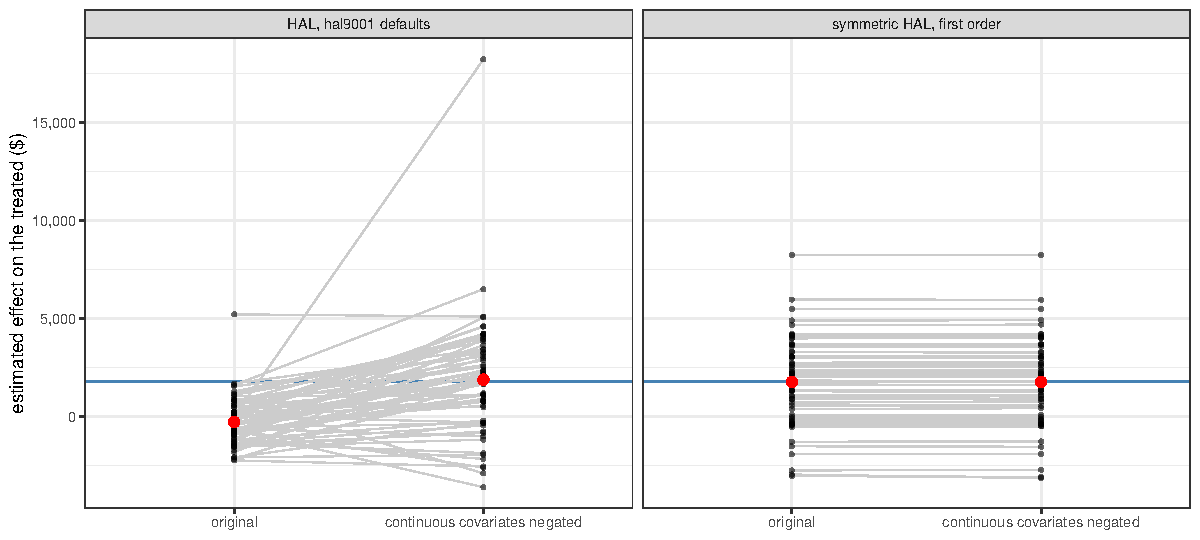
\includegraphics[width=\textwidth]{../figures/semisynth.pdf}
\caption{Semi-synthetic LaLonde: estimates of the effect on the treated in
66 replicates, under the original coding and with the continuous covariates
negated; lines join the two estimates from the same replicate. Blue: the
true effect, \$1{,}800; red: the mean.}
\label{fig:semisynth}
\end{figure}

\section{Discussion}

HAL's anchor is a convention of the variation norm that became a modelling
choice. It is invisible in the usual statement of HAL's rates, which are
uniform over a variation ball and so hide how large the ball has to be for
a given function; Proposition~\ref{prop:box} shows that for simple
functions the radius changes by a factor of up to $2^D - 1$ with the
coding. Symmetric HAL removes the dependence at a constant-factor cost in
dictionary size and none in rate.

In prediction the coding mostly shifts error around: symmetric HAL is not
more accurate than a typical coding of HAL, and on boxes that face HAL's
anchor it is somewhat worse. In causal estimation the coding can matter
more, because the nuisance errors enter the estimate as a bias the standard
error does not see. In the semi-synthetic LaLonde data the default
\texttt{hal9001} estimator under the original coding has a standard
deviation half the efficiency bound and a bias larger than that standard
deviation, so its intervals are tight and wrong; one sign flip of the
continuous covariates turns it into a nearly unbiased but noisier
estimator. Neither the analyst nor the reported standard error can tell
which of the two they have. Symmetric HAL gave an unbiased estimator near
the bound in both codings. That is one design with one effect, and
removing a dependence on coding does not settle the other specification
choices, the knot rule, the degree, the propensity cap, that the LaLonde
literature shows estimates are sensitive to \citep{smith2005}. It does
remove a choice that no analyst knows they are making. Where HAL feeds a
causal estimate, symmetric HAL is the more defensible default.

\clearpage
\bibliographystyle{apalike}
\bibliography{refs}

\clearpage
\appendix
\renewcommand{\thefigure}{\thesection\arabic{figure}}
\renewcommand{\thetable}{\thesection\arabic{table}}
\counterwithin*{figure}{section}
\counterwithin*{table}{section}
\section{All methods}\label{app:methods}

Figure~\ref{fig:all_methods} shows the median risk of every method in the
simulations of Section~\ref{sec:sims}, with the interquartile range across
replicates.

\begin{figure}[!h]
\centering
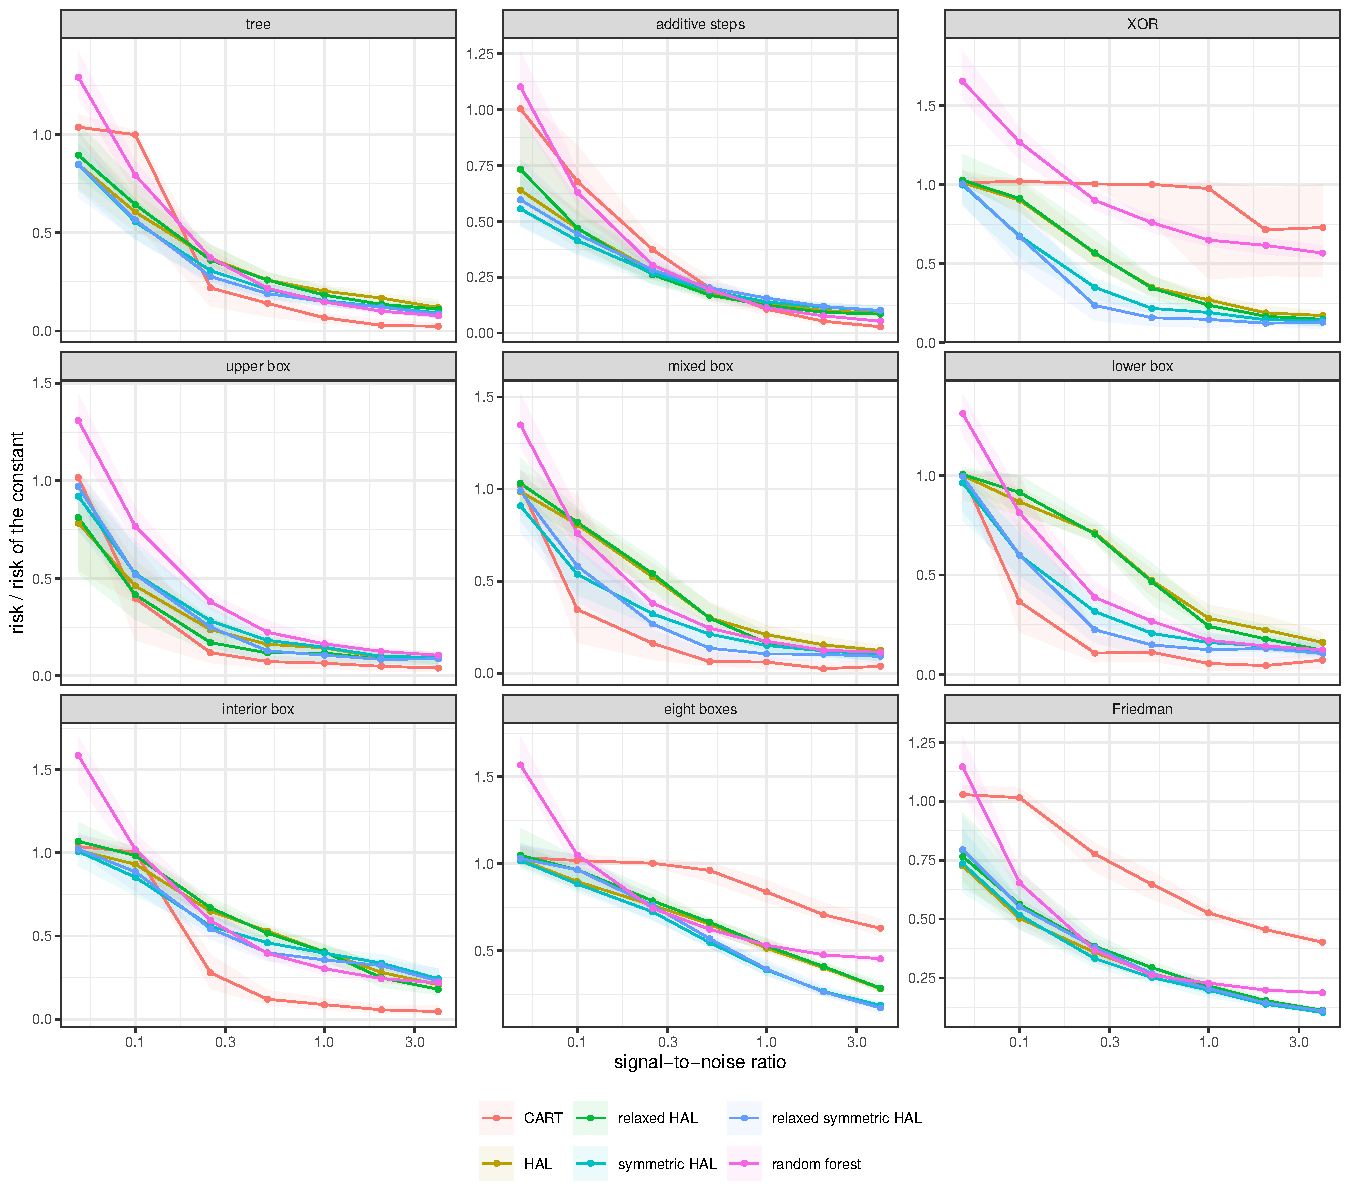
\includegraphics[width=\textwidth]{../figures/tier1_risk_vs_snr.pdf}
\caption{Median risk relative to the constant predictor (lines) and its
interquartile range across 50 replicates (bands), by true function and
signal-to-noise ratio.}
\label{fig:all_methods}
\end{figure}

\end{document}
